

\section{Understandability Study (RQ1)}
\label{sec:rq1}
This study presents programmers with regexes and asks comprehension questions. By comparing the understandability of semantically equivalent regexes that match the same language but have different syntactic representations, we aim to identify understandability code smells.
This study was implemented on Amazon's Mechanical Turk with 180 participants. A total of 60 regexes were evaluated, constructing 42 pairs of regex comparison. Each regex pattern was evaluated by 30 participants.
%The patterns used were designed to belong to various representations in Figure~\ref{fig:refactoringTree}.







\subsection{Metrics}
\label{sec:understadningmetric}
 We measure the understandability of regexes using two complementary metrics, \emph{matching} and \emph{composition}. These are referred to as the \emph{comprehension metrics}.
For a deeper look at the data to gain a better understanding of factors that impact comprehension, we also compute \emph{regex length} and \emph{DFA size} for each regex.


\textbf{Matching:}
 Given a pattern and a set of strings, a participant determines by inspection which strings will be matched by the pattern. There are four possible responses for each string, \emph{matches}, \emph{not a match}, \emph{unsure}, or blank. An example\footnote{Task instructions are also available: \url{https://github.com/wangpeipei90/RegexSmells/blob/master/questionnaire.pdf}} from our study is shown in Figure~\ref{fig:exampleQuestion}.

 The percentage of correct responses, disregarding blanks and unsure responses, is the matching score.
 For example, consider regex pattern \verb!`RR*'!, the five strings shown in Table~\ref{matchingmetric}, and the responses from four participants in the \emph{P1}, \emph{P2}, \emph{P3} and \emph{P4} columns.
 The {\em Oracle} indicates the first three strings match and the last two do not; 
 %Python's {\tt  re.search()} function is used to determine a match. 
 \emph{P1} answers correctly for the first three strings and the fifth, but incorrectly on the fourth, so the matching score is $4/5 = 0.80$. \emph{P2} incorrectly thinks that the second string is not a match, so the score is also $4/5 = 0.80$. \emph{P3} marks `unsure' for the third string and so the total number of attempted matching questions is 4. \emph{P3} is incorrect about the second and fourth string, so they score $2/4 = 0.50$. For \emph{P4}, we only have data for the first and second strings, since the other three are blank. \emph{P4} marks `unsure' for the second string so only one matching question has been attempted; the matching score is $1/1 = 1.00$.

Blanks were incorporated into the metric because questions were occasionally left blank in the study. Unsure responses were provided as an option so not to bias the results through blind guessing. These situations did not occur very frequently.
%Only 1.1\% of the responses were left blank and only 3.8\% of the responses were marked as unsure. %We refer to a response with all blank or unsure responses as an `NA'.
Out of 1,800 questions (180 participants * 10 questions each), only 1.8\%(32) were impacted by a blank or unsure response (never more than four out of 30 responses per pattern).


\begin{figure}[tb]
\centering
%\includegraphics[width=0.75\columnwidth]{illustrations/ExampleQuestion}
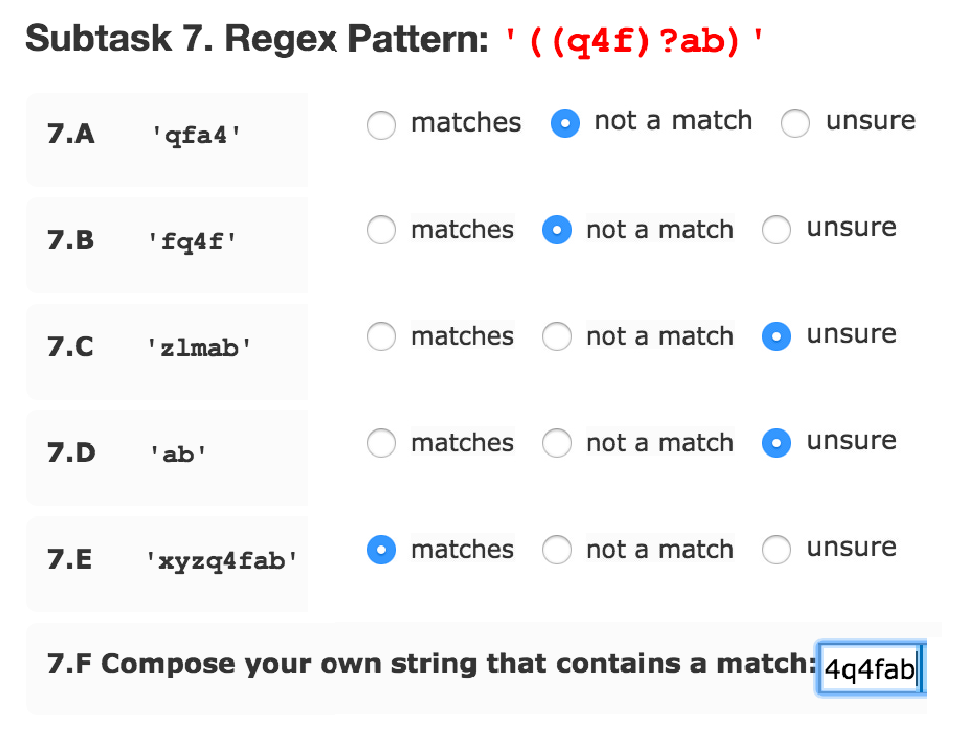
\includegraphics[width=0.75\columnwidth]{illustrations/exampleQuestion.eps}
\vspace{-12pt}
\caption{Questions from one pattern in one HIT}
\vspace{-6pt}
\label{fig:exampleQuestion}
\end{figure}



\begin{table} [t]
\caption{Matching metric example \label{matchingmetric}}
\begin{center}
%\begin{small}
\begin{tabular} {|cl | c c c c c|} \hline
\textbf{String} & \verb!`RR*'! & \textbf{Oracle} & \textbf{P1} & \textbf{P2} & \textbf{P3}& \textbf{P4}\\ \hline
1 & ``ARROW"    & \checkmark    & \checkmark    & \checkmark    & \checkmark    & \checkmark \\
2 & ``qRs"      & \checkmark    & \checkmark    & \xmark        & \xmark        & ?\\
3 & ``R0R"      & \checkmark    & \checkmark    & \checkmark    & ?             & -\\
4 & ``qrs"      & \xmark        & \checkmark    & \xmark        & \checkmark    & -\\
5 & ``98"       & \xmark        & \xmark        & \xmark        & \xmark        & -\\
\hline
  & Score       & 1.00          & 0.80          & 0.80          & 0.50          & 1.00\\ \hline
%\multicolumn{7}{l}{}\\
\multicolumn{7}{l}{\checkmark = match, \xmark = not a match, ? = unsure, -- = left blank}\\
\end{tabular}
%\end{small}
\end{center}
\vspace{-6pt}
\vspace{-6pt}
\end{table}



\textbf{Composition:}
Given a pattern, a participant composes a string they think it matches (question 7.F in Figure~\ref{fig:exampleQuestion}). If the participant is accurate, a composition score is 1, otherwise 0. For example, given the pattern \verb!(q4fab|ab)! from our study, the string, ``xyzq4fab" matches and gets a score of 1, but the string, ``acb" does not match and gets a score of 0.

%To determine a match, each pattern was compiled using the \emph{java.util.regex} library. A \emph{java.util.regex.Matcher} \verb!m! object was created for each composed string using the compiled pattern. If \verb!m.find()! returned true, then that composed string was a match and scored 1, otherwise it scored 0.
%To determine a match, each pattern was compiled using the \emph{java.util.regex} library in Java. A {\em java.util.regex.Matcher} \verb!m! was created for each composed string using the compiled pattern. If {\tt m.find()} returns {\tt true}, then that composed string was a match and scored 1; otherwise it scored~0.

%To determine a match, each pattern was compiled using the \emph{re.compile} module in Python. A regular expression object \verb!m! was created using the compiled pattern. \verb!m.search()! returns a regular match object \verb!m2! with the composed string as the input of the function. If \verb!m2! is not \emph{None}, then that composed string was a match and scored 1; otherwise it scored~0.
To determine the match between a string and a pattern, the pattern was compiled using the \emph{re.compile} module in Python. An object of \emph{re.RegexObject} \verb!m! was created using the compiled pattern. \emph{m.search()} returns an object of \emph{re.MatchObject} \verb!m2! with the string given as the input to this function. If \verb!m2! is not \emph{None}, then that string was a match and scored 1; otherwise it scored~0.

\textbf{Regex Length:}
Given a pattern, the regex length is computed by its literal string length. For example, regexes \verb!\072! and \verb!ab*c! are both length four.

\textbf{DFA Size:}
To compute the size of minimal DFA, we run both \textit{brics}~\cite{brics} and \textit{Rex}~\cite{rex} on each regex, and manually check their results to guarantee their correctness.
%The DFA size is the number of states of minimal DFA. We run both \textit{brics}~\cite{brics} and \textit{Rex}~\cite{rex} on each regex in order to get the minimal DFA. We also mannually check their results to guarantee their correctness.
\iffalse
We note that \textit{brics} always shows the minimal DFAs but its syntax is very restricted in language coverage~\cite{chapman2016} while \textit{Rex} accepts most regular expression features, but does not guarantee a minimal DFA (although, as it turns out, most are minimal). %Although most of the DFAs generated by \textit{Rex} are minimal but they are not guaranteed to be minimal.
For the regexes that are accepted by both \textit{brics} and \textit{Rex}, we chose the size of DFA generated from \textit{brics}. For example, the DFA size got from \textit{brics} for {\tt RR*} is two while the size from \textit{Rex} is three; thus, we select the smaller one.
For the regexes only accepted by \textit{Rex}, we examined the generated DFAs manually and made minor changes to make sure we use the minimal one. {\tt tuv$\backslash$w} and {\tt [a-f]($\backslash$d+)[a-f]} are only accepted by \textit{Rex} because {\tt $\backslash$w} and {\tt $\backslash$d} are not valid in \textit{brics}. While the DFA sizes for both regexes from \textit{Rex} are five, we set the DFA size of {\tt tuv$\backslash$w} to five and the DFA size of {\tt [a-f]($\backslash$d+)[a-f]} to four. This is because the DFA of the former is minimal but that of the latter is not minimal and could be reduced.
\fi
\subsection{Design}
%\todoNow{needs to be updated with respect to no C1,  T1 nodes}
We implemented this study on Amazon's Mechanical Turk (MTurk), a crowdsourcing platform where requesters create human intelligence tasks (HITs) for completion by workers.
%Each HIT is designed to be completed in a fixed amount of time and workers are compensated with money if their work is satisfactory. Requesters can screen workers by requiring each to complete a qualification test prior to completing any HITs.

\subsubsection{Worker Qualification}
Workers qualified to participate by answering questions regarding some basics of regex knowledge. These questions were multiple-choice and asked the worker to analyze the following patterns: \verb!a+!, \verb!(r|z)!, \verb!\d!, \verb!q*!, and \verb![p-s]!. To pass the qualification test, workers had to answer four of the five questions correctly.

\subsubsection{Tasks}
Using the patterns in the corpus as a guide, we created 60 regex patterns that were grouped into 26 semantic equivalence groups.
 There were 18 groups with two regexes that target various edges in the equivalence classes.
The other eight semantic groups had three regexes each, forming 42 total pairs.
These semantic groups were intended to explore edges in the equivalence classes. In this way, we can draw conclusions by comparing between representations since the regexes evaluated were semantically equivalent.

To form the semantic groups, we took a regex from the corpus, matched it to a representation in Figure~\ref{fig:refactoringTree}, trimmed it down so it contained little more than just the feature of interest, and then created other regexes that are semantically equivalent but belong to other nodes in the equivalence class. For example, a semantic group with regexes \verb!((q4f){0,1}ab!, \verb!((q4f)?ab)!, and \verb!(q4fab|ab)! belong to D1, D2, and D3, respectively.
A group with regexes \verb!([0-9]+)\.([0-9]+)! and \verb!(\d+)\.(\d+)! is intended to evaluate the edge between C1 and C4.
We note that if we only used regexes from the corpus, we would have had regexes with different semantics at each node, or with additional language features, which would make the comparisons of the targeted features difficult.




%Using the patterns in the corpus as a guide, we created six metagroups containing three pairs of patterns focusing on:
%\begin{itemize}
%\item S1 vs S2
%\item the digit default character class vs C1
%\item the word default character class vs C1
%\item negated digits and words vs C3, whitespace vs C2
%\item additional vs Kleene repetition
%\item wrapping vs escaping literal characters
%\end{itemize}
%and four metagroups containing two triplets of patterns focusing on
%\begin{itemize}
%\item octal vs hex vs literal
%\item D1 vs D2 vs D3
%\item C1 vs C2 vs C5
%\item octal vs literal and C2 vs C5
%\end{itemize}
%
%Each of these 10 metagroups contains 6 strings, resulting in a total of 60 regex patterns. These patterns are logically partitioned into 26 semantic equivalence groups (18 from pairs, 8 from triples).





For each of the 26 semantic groups, we created five strings for the study, where at least one matched and at least one did not match. These were used to compute the matching metric.

Once all the patterns and matching strings were collected, we created tasks for the MTurk participants as follows:
randomly select a pattern from 10 of the 26 semantic groups. Randomize the order of these 10 patterns, as well as the order of the matching strings for each pattern. After adding a question asking the participant to compose a string that each pattern matches, this creates one task on MTurk, such as the example in Figure~\ref{fig:exampleQuestion}. This process was completed until each of the 60 regexes appeared in 30 HITs, resulting in a total of 180 total unique HITs.
%An example of a single regex pattern, the five matching strings and the space for composing a string is shown in



\subsubsection{Implementation}
Workers were paid \$3.00 for successfully completing a HIT, and were only allowed to complete one HIT. The average completion time for accepted HITs was 682 seconds (11 mins, 22 secs).
%A total of 241 HITs were submitted - of those 55 were rejected.
% and 6 duplicates were ignored, always using the first accepted submission so as to obtain a value for each of the 180 distinct tasks.
A total of 54 HITs were rejected: 48 had too many blank responses, four were double-submissions by the same worker, one did not answer the composition questions, and one was missing data for 3 questions. Rejected HITs were returned to MTurk to be completed by others.


%
%
%
%\begin{figure}[tp]
%\begin{small}
%\fbox{\parbox{\columnwidth}{
%\begin{enumerate}
%\item
%\begin{tabular} {lrr}
%\textbf{What is your gender?} & \textbf{n} & \textbf{\%}\\ \hline
%Male & 149 & 83\%\\
%Female & 27& 15\%\\
%Prefer not to say & 4& 2\%
%\end{tabular}
%\item \textbf{What is your age?} \\
%$\mu = 31$, $\sigma = 9.3$
%
%\item
%
%\begin{tabular} {l |rr}
%\textbf{Education Level?} & \textbf{n} & \textbf{\%}\\ \hline
%High School & 5 & 3\%\\
%Some college, no degree & 46 & 26\%\\
% Associates degree & 14 & 8\%\\
%Bachelors degree & 78 & 43\%\\
%Graduate degree & 37 & 21\%\\
%\end{tabular}
%\item
%\begin{tabular} {lrr}
%\textbf{Familiarity with regexes?} & \textbf{n} & \textbf{\%}\\ \hline
%Not familiar at all & 5 & 3\%\\
%Somewhat not familiar & 16 & 9\%\\
%Not sure & 2 & 1\%\\
%Somewhat familiar & 121 & 67\%\\
%Very familiar & 36 & 20\%\\
%\end{tabular}
%\item \textbf{How many regexes do you compose each year?} \\
%$\mu = 67$, $\sigma = 173$
%\item \textbf{How many regexes (not written by you) do you read each year?} \\
%$\mu = 116$, $\sigma = 275$
%%\item In what contexts do you use regexes? \\
%\end{enumerate}
%}}
%\caption{Participant Profiles, $n=180$ \todoLast{can remove this for space} \label{participantprofile}}
%\end{small}
%\end{figure}
%


\subsubsection{Participants}

In total, there were 180 participants.
A majority were male (83\%). % with an average age of 31.
Most had
at least an Associates degree (72\%), were at least somewhat familiar with regexes (87\%), and have prior programming experience (84\%).
%On average,
%participants compose 67 regexes per year with a range from 0 to 1000.
%Participants read more regexes than they write with an average of 116 and a range from 0 to 2000.
%Figure~\ref{participantprofile} summarizes the self-reported participant characteristics from the qualification survey.


%\todoNow{in study section present choices about pairwise vs random selection for nodes.}



\begin{table}[t]
\centering
\caption{3-factor ANOVA with average matching or composition accuracy as dependent variables, considering representation (rep), DFA size (dfa\_size), and regex length (len) as independent variables}
\begin{tabular}{@{}l@{}r|rl|ll@{}}

  \multicolumn{2}{c}{} & \multicolumn{2}{c}{Average Matching} & \multicolumn{2}{c}{Average Composition} \\
    \hline
 & Df & F value & Pr($>$F) & F value & Pr($>$F) \\
  \hline
dfa\_size &              1 &  7.632 &0.0153 * & 10.084 &0.00674 ** \\
len      &          1 &  3.325 &0.0896 $\cdot$ &  0.001 &0.98161 \\
rep            &      15 &  2.062 &0.0921 $\cdot$ & 1.224 &0.35538\\
dfa\_size:len  &     1 & 1.002 &0.3339  & 1.384 &0.25907   \\
dfa\_size:rep    &     14 & 0.709 &0.7355 &0.920& 0.56075   \\
len:rep     &     10 & 0.924& 0.5397  &  0.599& 0.79054   \\
dfa\_size:len:rep  &3&  1.163& 0.3589 & 0.678 &0.58002   \\
Residuals        &     14&&&&\\
   \hline
\end{tabular}

\vspace{3pt}
$\cdot\alpha = 0.10$ \hspace{3pt} *$\alpha=0.05$ \hspace{3pt} **$\alpha=0.01$ \hspace{3pt} ***$\alpha=0.001$
%The F values and p values in column 3-4 are of ANOVA results with average matching accuracy as dependent variables. These values in column 5-6 are for ANOVA results with composition accuracy.
\label{table:anova}
\end{table}

\iffalse
\begin{table}[t]
\centering
\caption{3-factor ANOVA results with average composition accuracy as the dependent variable, considering representation (rep), DFA size (dfa\_size), and regex length (len) as independent variables}
\begin{tabular}{@{}l@{}rrrrl@{}}
  \hline
 & Df & Sum Sq & Mean Sq & F value & Pr($>$F) \\
  \hline
dfa\_size     &          1 &  3548 &   3548 & 10.084 &0.00674 **\\
len     &           1    &  0    &   0 &  0.001 &0.98161 \\
rep              &    15   &6458  &   431  & 1.224 &0.35538\\
dfa\_size:len   &    1   & 487   &  487  & 1.384 &0.25907   \\
dfa\_size:rep     &    14  & 4532    & 324   &0.920& 0.56075   \\
len:rep     &     10  & 2107&     211 &  0.599& 0.79054   \\
dfa\_size:str:rep & 3  &  715 &    238  & 0.678 &0.58002   \\
Residuals          &   14  & 4926  &   352  &&\\
   \hline
\end{tabular}

\vspace{3pt}
.$\alpha = 0.10$ \hspace{3pt} *$\alpha=0.05$ \hspace{3pt} **$\alpha=0.01$ \hspace{3pt} ***$\alpha=0.001$
\label{table:anova2}
\end{table}
\fi

\begin{table*}\begin{small}\begin{center}\caption{Averaged Info About Edges}\label{table:testedEdgesTable}\begin{tabular}
{llccccccc}
index & edge & nExp & acc1 & acc2 & cmp1 & cmp2 & Pacc & Pcmp \\
\toprule[0.16em]
E1 & C1 -- C2 & 2 & 0.94 & 0.90 & 28.0 & 27.0 & 0.268800 & 0.802400\\
E2 & C1 -- C2, T2  -- T1 & 2 & 0.84 & 0.86 & 19.5 & 27.5 & 0.751200 & 0.031185\\
E3 & C1 -- C2,T4->T1 & 2 & 0.81 & 0.86 & 15.5 & 27.5 & 0.609700 & 0.022661\\
E4 & C1->C4 & 5 & 0.76 & 0.76 & 24.2 & 23.8 & 0.555860 & 0.500942\\
E5 & C1->C5 & 5 & 0.90 & 0.88 & 27.0 & 27.2 & 0.472560 & 0.551300\\
E6 & C2->C4 & 1 & 0.83 & 0.92 & 18.0 & 20.0 & 0.075020 & 0.788800\\
E7 & C2->C5 & 4 & 0.85 & 0.86 & 26.5 & 28.5 & 0.282075 & 0.598075\\
E8 & C2->C5,T4->T1 & 2 & 0.60 & 0.82 & 11.0 & 29.0 & 0.048688 & 0.000015\\
E9 & D1->D2 & 2 & 0.84 & 0.78 & 28.0 & 26.5 & 0.306450 & 0.598350\\
E10 & D1->D3 & 2 & 0.84 & 0.87 & 28.0 & 29.0 & 0.526250 & 0.802400\\
E11 & D2->D3 & 2 & 0.78 & 0.87 & 26.5 & 29.0 & 0.155290 & 0.598350\\
E12 & L2->L3 & 3 & 0.86 & 0.91 & 27.3 & 29.3 & 0.230233 & 0.751533\\
E13 & S1->S2 & 3 & 0.86 & 0.85 & 27.0 & 26.3 & 0.420767 & 1.000000\\
E14 & T1->T3 & 3 & 0.88 & 0.86 & 21.7 & 22.7 & 0.177233 & 0.697267\\
E15 & T1->T4 & 2 & 0.80 & 0.60 & 26.0 & 11.0 & 0.049250 & 0.002759\\
E16 & T2->T4 & 2 & 0.84 & 0.81 & 19.5 & 15.5 & 0.519000 & 0.535040\\
\bottomrule[0.13em]\end{tabular}\end{center}\end{small}\end{table*}


\subsection{Analysis}
We computed a matching and composition score for each regex based on the 30 participant responses.
The average analysis or average composition is computed by averaging the associated 26-30 values for each metric for each of the 60 regexes (fewer than 30 values were used if all the responses in a matching question were a combination of blanks and unsure). %Next, we computed average scores for matching and composition per regex.
%\todoLast{Mentioning NAs here?}


%Each regex was a member of one of 26 groupings of equivalent regexes.
%These groupings allow pairwise comparisons of the metrics values to determine which representation of the regex was most understandable and the direction of a refactoring for understandability.
Of the original 42 pairs, we report scores for 41. Due to a design flaw, the regexes evaluated, \verb!\..*! and \verb!\.+!. were not semantically equivalent (the former is missing an escape and should be \verb!\.\.*!), so this was omitted from the data. In the end, we analyzed 58 regexes that cover 17 edges from Figure~\ref{fig:refactoringTree}.

To gain a better understanding of why some regexes may be more understandable than others, we also look at the impact of the representation from Figure~\ref{fig:refactoringTree}, regex length, and DFA size\footnote{Note that the study was not specifically designed for regex length and DFA size} on the comprehension metrics.
Note that we retain all 60 regexes for this analysis as we are looking at the properties of regexes individually.
We conduct two three-factor analysis of variances (ANOVAs) with matching accuracy and composition accuracy as the dependent variables.
We also conduct the correlation analysis between these three factors and the composition metrics.
We use Spearman's Rank-Order Correlation because we have no priori knowledge about the distributions of the factors.
Since the regex representations are categorical data, these are excluded from the correlation analysis.



\subsection{Results}
The ANOVA in Table~\ref{table:anova} shows that DFA size significantly affects both the average matching accuracy and the average composition at $\alpha = 0.05$ and $\alpha = 0.01$, respectively.
The length and representation from Figure~\ref{fig:refactoringTree} each significantly affect the average matching accuracy at $\alpha = 0.10$.
Since the DFA sizes vary across the pairwise comparisons within a representation, we present our results for matching and composition using each of the 41 pairs of regexes separately, rather than in aggregate over the equivalence class edges explored. %



%\textcolor{red}{Todo: update Table and its description, add annova and correlation analysis about representation, dfa size, and string length}

For the comprehension metrics, Table~\ref{table:testedEdgesTable} presents the results.
Each row represents a {\em Pair} of regex evaluated by study participants.
The representations for the regexes per Figure~\ref{fig:refactoringTree} are shown in the {\em Edge} column, which is how the table is sorted.
The {\em Regex 1} and {\em Regex 2} columns identify the regexes used in the study, mapping to the first and second representations in the {\em Edge} column, respectively.
{\em Match1} is the average matching for {\em Regex 1} and {\em Match2} is the average matching for {\em Regex~2}.
Using the Mann-Whitney test of means, the {\em sigM} column following tests if there is a significant difference between the accuracies.
The {\em Comp1} column presents the percentage of the string responses for that were in fact correctly matched by {\em Regex 1}. {\em Comp2} presents the same information, except for {\em Regex 2}.
The following {\em sigC} column uses a test of two proportions to identify if the percentage of the participants who correctly composed a string for Regex 1 is significantly different than the percentage who correctly composed a string for {Regex 2}.


%, \emph{Nodes} lists the representations, \emph{Pairs} shows the number of comparisons, \emph{Example Preferred Regex} shows a regex from the preferred node (bolded in \emph{Pairs} column), \emph{Match1} and \emph{Match2} give the matching scores for the first and second representations, respectively, and $H_0: \mu_{match1} = \mu_{match2}$ uses the Mann-Whitney test of means to compare the matching scores, and presents the p-values. The last three columns list the average composition scores for the representations and the composition p-value.

To illustrate, consider pair 16 in Table~\ref{table:testedEdgesTable}.
One pair of regexes was \verb!([}{])! and \verb!(\{|\})! in C4 and C5, respectively, with average matching scores of 78.79\% and 70.33\% and average composition scores of 50.00\% and 86.67\%, respectively.
The difference between the composition scores is significant at $\alpha = 0.01$, yet the difference between the accuracies is not.
In fact, the representation C5 was more understandable in that participants could more effectively compose a string that it would match, but C4 is more understandable in that participants could more easily determine which of a set of strings would be matched by C4. Thus, neither representation is bolded in the \emph{Edge} column since there is a conflict.
If both comprehension metrics indicated a preferred representation, that representation is bolded (e.g., C4 in pair 15). Ties are broken by deferring to the other metric (e.g., there's a tie in composition for row 17, but matching indicates a preference for C5, so C5 is bolded).
%Thus, the community found \verb!R+! from L3 more understandable.
%This is not the only regex pair in E5, however, The other is \verb!zaa*! and \verb!za+!. %, and regexes pair \verb!\..*! and \verb!\.+'!.
%In aggregate, considering both regex pairs, the overall matching average for the regexes belonging to L2 was 0.86 and 0.91 for L3.
%The overall composition score for L2 was 0.97 and 1.00 for L3.
%The community found L3 to be more understandable than L2, from the perspective of both metrics, suggesting that L2 is generally smelly, though the differences are not significant.


%
%\begin{figure}[tb]
%\centering
%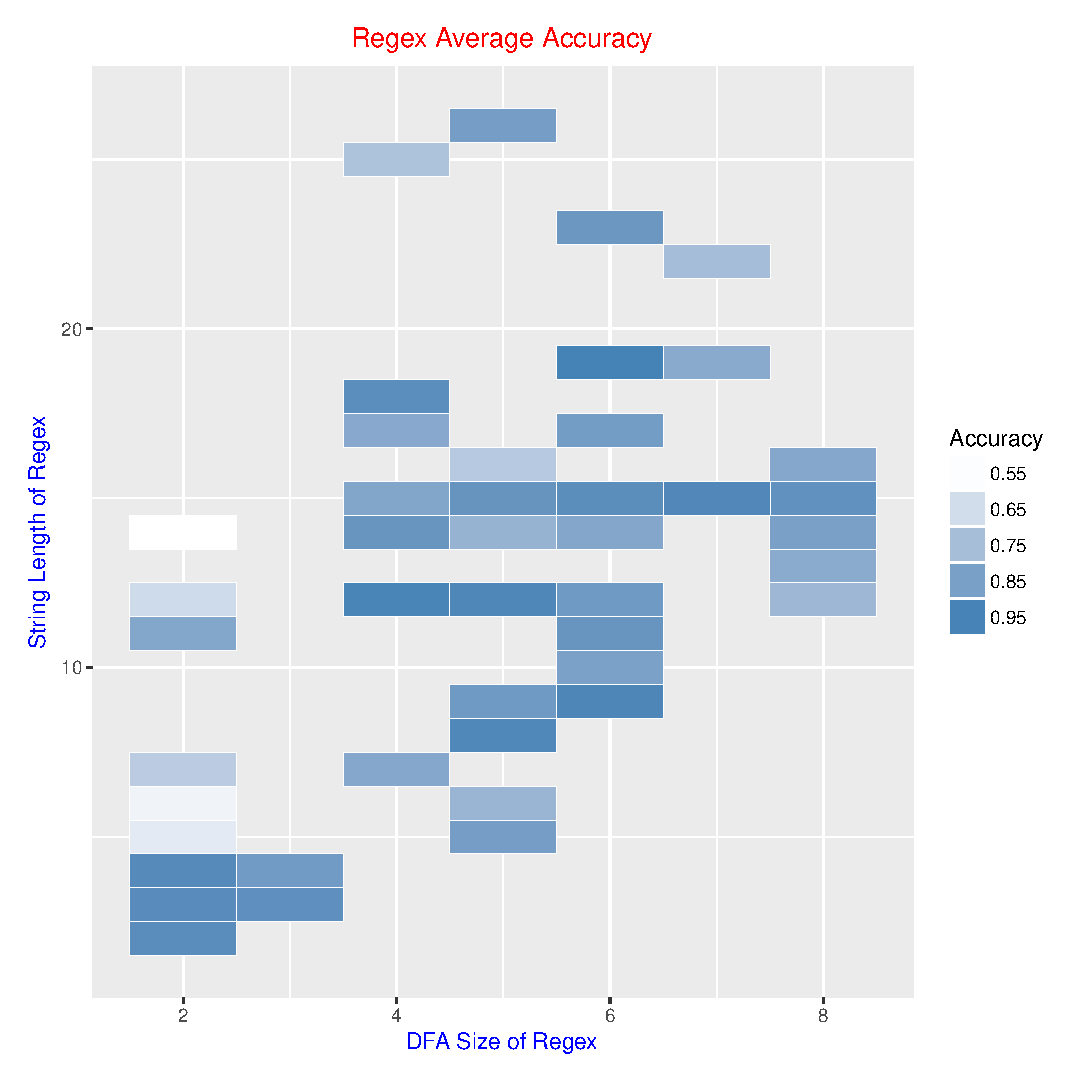
\includegraphics[width=0.75\columnwidth]{graphs/heatmap_avgAccur.eps}
%\vspace{-12pt}
%\caption{Heatmap for impacts of DFA size and regex string length on accuracy/matching}
%\vspace{-6pt}
%\label{fig:heatmap}
%\end{figure}

%60 strings
%42 comparisons
%18@2, 8@3
%
%M6R1 ? group 3, 3 comparisons
%- 1 comparisons
%- 0 strings
%
%M3R0 ? group 3, 3 comparisons
%- 1 comparisons
%- 0 strings
%
%M3R1 ? group 3, 3 comparisons
%- 2 comparisons
%- 1 string
%
%M3R0 ? group 3, 3 comparisons
%- 2 comparisons
%- 1 string
%
%58 strings
%36 comparisons


%Although we performed 42 pairwise comparisons,

%\subsection{Results}
% In E1 through E4, there is a statistically significant difference between the representations for at least one of the metrics with $\alpha = 0.10$. These represent the strongest evidence for code smells, suggesting that T4, D2, and C2 are less understandable.

For pairs 16, 29, 34, and 36, the difference in composition is significant at $\alpha < 0.05$, indicating differences favoring C5 over C4, T1 over T2, and twice favoring T1 over T4.
For pairs 23, 37, and 38, the difference in matching is significant with $\alpha < 0.05$, indicating differences favoring D3 over D2 and twice favoring T1 over T4.
%There appears to be a clear trend favoring T1 over T4.
Interestingly, for pairs 16 and 29, while the differences in composition are significant, there is a conflict between the composition metrics. Further investigation is needed to understand in what circumstances the metrics are in conflict with one another.


% and we can use that to further corroborate the understandability analysis.

%\begin{table*}
%\centering
%\caption{Average Unsure Responses Per Pattern By Node (fewer unsures on the left)}\label{table:unsureResults}
%\begin{tabular}{|| l || cccc || cccc || || cccc || cccc ||}
%                & \multicolumn{4}{c||}{>=Q0(0.67)}         & \multicolumn{4}{c||||}{>=Q1(1.25)}   & \multicolumn{4}{c||}{>=Q2(1.94)}    &  \multicolumn{4}{c||}{>=Q3(2.54)}  \\ \hline
%Node     & L3 & D3 & C2 & C1 & L2 & S2 & S1 & C4 & D1 & C5 & C3 & D2 & T1 & T3 & T2 & T4 \\
%% Number of Patterns - reversed & 4 & 2 & 3 & 3 & 2 & 2 & 4 & 2 & 9 & 3 & 3 & 3 & 8 & 5 & 2 & 3\\
%Unsure Responses Per Pattern & 0.7 & 1 & 1 & 1 & 1.3 & 1.7 & 1.7 & 1.9 & 2 & 2 & 2 & 2.5 & 2.7 & 2.7 & 5.5 & 8.5\\
%\end{tabular}
%\end{table*}
Recall that participants were able to select \emph{unsure} for whether a string is matched by a pattern.
From a comprehension perspective, this indicates some level of confusion.
For each pattern, we counted the number of responses containing at least one unsure.
%We then grouped the patterns into their representation nodes and computed an average of unsures per pattern.
%A higher number may indicate difficulty in comprehending a pattern from that node.
Overall, the highest number of unsure responses came from T4 and T2, which have octal and hex representations of characters. The least number of unsure responses were in L3 and D3.
%, which are both shown to be understandable by looking at E2 and E3 in Table~\ref{table:testedEdgesTable}.
%These nodes and their average number of unsure responses are organized by quartile in Table~\ref{table:unsureResults}.
These results mirror the understandability analysis, as T4 and T2 are generally lower in comprehension, and L3 and D3 are generally higher.%, echoing that L3 and D3 are less smelly.
% for the LIT group (i.e., $\overrightarrow{T4 T1}$), the DBB group (i.e., $\overrightarrow{D2 D3}$), and the LWB group (i.e., $\overrightarrow{L2 L3}$) because the more understandable node has the least unsures of its group.
% The findings for D3 and D2 are contradictory, however, as and further study is needed.
% and the number of unsures may be too small to indicate anything, except for T2 and T4. The one pattern from T4 that had the most unsures of any pattern (i.e., 10 out of 30) was \verb!`xyz[\0133-\0140]'!, so this may have been the least understandable pattern that we tested.

While the ANOVA indicates that variance in matching is due to all three factors, representation, DFA size, and regex length, it is not entirely clear why. Variance in composition is impacted by DFA size only.
Between DFA size and composition, there is a strong, positive correlation at $\alpha = 0.01$ with $\rho = 0.354$.
%Between regex length and accuracy, Spearman's $\rho=-0.025$, indicating a weak negative relationship.
%For DFA size the accuracy, the correlation is weak and positive $\rho=0.07$.
At first, this result may seem counter-intuitive, but considering that larger DFAs may represent more constrained regex languages (i.e., languages that accept fewer strings), these may be easier to compose a string for.
However, as the explored DFA size range was between two and eight nodes, these results may not generalize to larger regexes.
None of the other correlations are significant with $\alpha < 0.05$.%the regular language with a relatively small scope and thus easier for people to recognize.


%Figure~\ref{fig:heatmap} is a heatmap showing the average matching accuracies of the 60 regexes along with their DFA sizes and string lengths.
%We see no clear trends considering these variables, though the ANOVA that both significantly impact the variance in the matching accuracy.
% the color is darker towards the bottom and left, which confirms the correlation analysis results. \todo{I'm not convinced that the heatmap provides enough value to keep in the paper.}
%We also note that since composition is either 1 or 0, we do not perform an ANOVA with composition as the dependent variable. \todo{is this the correct decision?}

\subsection{Summary}
Matching and composition are impacted by DFA size, and matching is also impacted by regex length and representation, showing some support that the representation of the regex impacts comprehension.
The larger the DFA, the easier it was for the community to generate strings that match it.
%, and regex length, illustrating no clear trends explaining why some regexes are more understandable than others, but we have some hints from the pairwise comparisons.
There also appears to be a clear trend favoring T1 over T4. Representations D3 and C5 are also preferred. While C1 is favored comparisons against C2, C4, and C5, none are significant.

%\todo{impact of size on matching, composition}
